\documentclass[10pt, a5paper]{article}
\usepackage{pdfpages}
\usepackage{parallel}
\usepackage[T2A]{fontenc}
\usepackage{ucs}
\usepackage[utf8x]{inputenc}
\usepackage[polish,english,russian]{babel}
\usepackage{hyperref}
\usepackage{rotating}
\usepackage[inner=2cm,top=1.8cm,outer=2cm,bottom=2.3cm,nohead]{geometry}
\usepackage{listings}
\usepackage{graphicx}
\usepackage{wrapfig}
\usepackage{longtable}
\usepackage{indentfirst}
\usepackage{array}
\newcolumntype{P}[1]{>{\raggedright\arraybackslash}p{#1}}
\frenchspacing
\usepackage{fixltx2e} %text sub- and superscripts
\usepackage{icomma} % коскі ў матэматычным рэжыме
\PreloadUnicodePage{4}

\newcommand{\longpage}{\enlargethispage{\baselineskip}}
\newcommand{\shortpage}{\enlargethispage{-\baselineskip}}

\def\switchlang#1{\expandafter\csname switchlang#1\endcsname}
\def\switchlangbe{
\let\saverefname=\refname%
\def\refname{Літаратура}%
\def\figurename{Іл.}%
}
\def\switchlangen{
\let\saverefname=\refname%
\def\refname{References}%
\def\figurename{Fig.}%
}
\def\switchlangru{
\let\saverefname=\refname%
\let\savefigurename=\figurename%
\def\refname{Литература}%
\def\figurename{Рис.}%
}

\hyphenation{admi-ni-stra-tive}
\hyphenation{ex-pe-ri-ence}
\hyphenation{fle-xi-bi-li-ty}
\hyphenation{Py-thon}
\hyphenation{ma-the-ma-ti-cal}
\hyphenation{re-ported}
\hyphenation{imp-le-menta-tions}
\hyphenation{pro-vides}
\hyphenation{en-gi-neering}
\hyphenation{com-pa-ti-bi-li-ty}
\hyphenation{im-pos-sible}
\hyphenation{desk-top}
\hyphenation{elec-tro-nic}
\hyphenation{com-pa-ny}
\hyphenation{de-ve-lop-ment}
\hyphenation{de-ve-loping}
\hyphenation{de-ve-lop}
\hyphenation{da-ta-ba-se}
\hyphenation{plat-forms}
\hyphenation{or-ga-ni-za-tion}
\hyphenation{pro-gramming}
\hyphenation{in-stru-ments}
\hyphenation{Li-nux}
\hyphenation{sour-ce}
\hyphenation{en-vi-ron-ment}
\hyphenation{Te-le-pathy}
\hyphenation{Li-nux-ov-ka}
\hyphenation{Open-BSD}
\hyphenation{Free-BSD}
\hyphenation{men-ti-on-ed}
\hyphenation{app-li-ca-tion}

\def\progref!#1!{\texttt{#1}}
\renewcommand{\arraystretch}{2} %Іначай формулы ў матрыцы зліпаюцца з лініямі
\usepackage{array}

\def\interview #1 (#2), #3, #4, #5\par{

\section[#1, #3, #4]{#1 -- #3, #4}
\def\qname{LVEE}
\def\aname{#1}
\def\q ##1\par{{\noindent \bf \qname: ##1 }\par}
\def\a{{\noindent \bf \aname: } \def\qname{L}\def\aname{#2}}
}

\def\interview* #1 (#2), #3, #4, #5\par{

\section*{#1\\{\small\rm #3, #4. #5}}

\def\qname{LVEE}
\def\aname{#1}
\def\q ##1\par{{\noindent \bf \qname: ##1 }\par}
\def\a{{\noindent \bf \aname: } \def\qname{L}\def\aname{#2}}
}

\switchlang{ru}
\begin{document}
\title{Создание робота для Roborace\footnote{\url{sklipus@gmail.com}, \url{http://lvee.org/ru/abstracts/163}}}
\author{Dmitry Sklipus, Brest, Belarus}
\maketitle
\begin{abstract}
Author shares his development experience of Arduino-based robots targeted at Roborace competitions. Specifics of the com\-petition is explained as far as some details of the hardware platform and the contol algorythm.
\end{abstract}
\subsection*{Специфика Roborace}

Roborace "--- это состязания, в которых соревнуются \linebreak роботы-автомобили на специальной кольцевой трассе. Можно провести некоторую аналогию между Roborace и гонками Формулы 1, за исключением двух моментов.

\begin{itemize}
  \item Во-первых, вместо полномасштабных гоночных болидов участвуют уменьшенные модели авто и оригинальные конструкции с габаритными и весовыми ограничениями (максимальные ШхД=25х50 см и вес до 3 кг).
  \item Во-вторых, вместо пилотов автомобилем управляет бортовой компьютер, который анализирует показания различных датчиков и ориентирует автомобиль на трассе, выбирает скорость движения, предотвращает столкновения с препятствиями и соперниками. Собственно “поведение” авто на трассе определяется управляющей программой бортового компьютера.
\end{itemize}

Roborace проводится в виде чемпионата, состоящего из этапов, которые организуются в различных городах Беларуси и за рубежом. Участие в чемпионате принимают как конструкции начального уровня (например, на базе конструктора типа LEGO), так и сложные робототехнические устройства. Регламенты соревнований формируются таким образом, чтобы охватить как можно более широкий спектр характеристик и возможностей робототехнических конструкций.


\begin{figure}[h!]
  \centering
  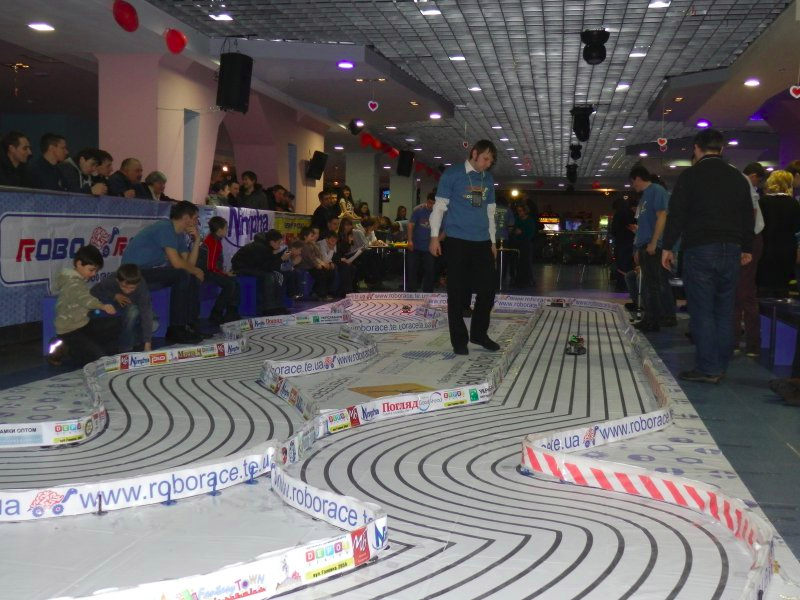
\includegraphics[width=10cm]{w_09_2016_Sklipus1.png}
  \caption {Трасса для гонок роботов}\label{Sklipus1}
\end{figure}

Рассмотрим трассу, изображенную на рисунке ~\ref{Sklipus1}, по которой предстоит перемещаться роботу. Обязательными элементами являются черные линии и стенки. Исходя из этого можно строить стратегию движения робота по трассе: например, оборудовать робота датчиками черной линии и использовать линии трассы для навигации, или установить дальномеры для обнаружения препятствий и двигаться вдоль стенок.

В рамках данной статьи представлен один из роботов, разработанный мной для Roborace по второй стратегия (движение на основе показаний дальномеров).

\subsection*{Этапы создания робота}

Создание робота для Roborace начинается с выбора шасси. Сейчас магазины предлагают большой выбор гусеничных и колесных платформ. Я рекомендую остановиться на классической схеме, когда задние колеса приводятся в движение электродвигателем, а передние управляются сервоприводом~\cite{Sklipus1}. На рисунке ~\ref{Sklipus2} изображен робот для Roborace, построенный по подобной схеме.

\begin{figure}[h!]
  \centering
  \includegraphics[width=5cm]{w_09_2016_Sklipus2.png}
  \caption {Робот}\label{Sklipus2}
\end{figure}

Мне повезло за небольшие деньги приобрести модель в местном клубе радио-моделистов (читатели могут попытаться сделать то же самое в своем регионе: обычно у них много устаревших моделей). Так как в приобретенной модели не было тягового электродвигателя, на нее был установлен установил купленный 12-вольтный мотор. Можно было также использовать обычную игрушку: они обычно довольно живучи, и требуется только модифицировать рулевое управление.

Так как в моем случае сервопривод уже был установлен, с ним проблем не возникло.

Следующий этап "--- выбор платы управления. Тут есть множество вариантов. Я выбрал Arduino как самый простой вариант. То же можно порекомендовать и читателю, особенно при недостатке опыта. Исходя из моего достаточно большого опыта, для таких роботов достаточно обычных 8-битных микроконтроллеров. Поэтому если не планируется использовать для отслеживания движений робота камеру, не стоит усложнять его более мощным процессором.

Сервопривод можно напрямую подключить к Arduino "--- например, через sensor shield, изображенный на рисунке ~\ref{Sklipus3}. К нему также удобно подключать датчики.

\begin{figure}[h!]
  \centering
  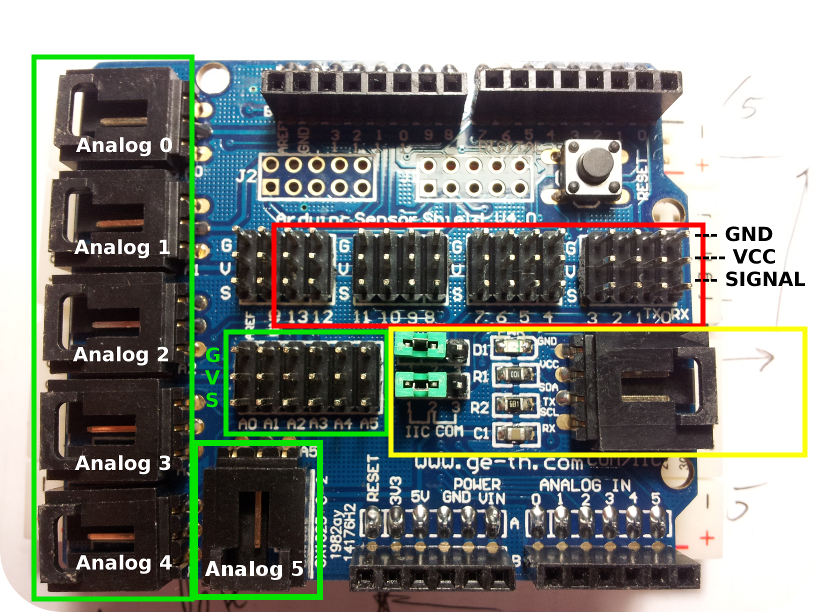
\includegraphics[width=7cm]{w_09_2016_Sklipus3.png}
  \caption {Sensor shield v4}\label{Sklipus3}
\end{figure}


Мотор подключить к Arduino напрямую не получится. Нужно использовать специальные Motor Driver. Сейчас из достаточно много в продаже, и есть инструкции по подключению. Я использовал Motor Driver, разработанный в нашей лаборатории (рис. ~\ref{Sklipus4}).

\begin{figure}[h!]
  \centering
  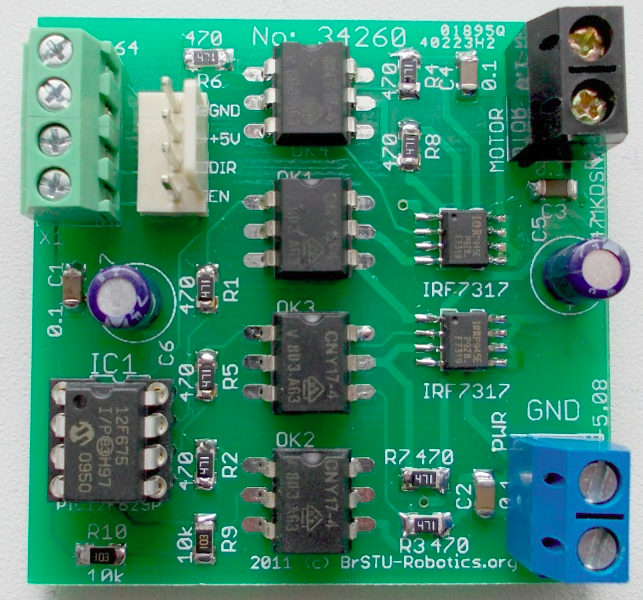
\includegraphics[width=7cm]{w_09_2016_Sklipus4.png}
  \caption {Motor driver}\label{Sklipus4}
\end{figure}


В соревнованиях роботов приходится много внимания уделять батареям. Я использую литий-полимерные аккумуляторы. Они \linebreak очень хорошо себя зарекомендовали. Один из хаков, которые я применяю в своем роботе, касается преобразователя напряжения. Штатный преобразователь в Arduino не очень хорош, поэтому для экономии энергии аккумулятора неплохо использовать Step-Down регулятор~\cite{Sklipus2}. Конечно, можно использовать и обычный линейный преобразователь.

Самая главная часть робота это датчики "--- то, что обеспечивает его информацией об окружающем мире, о препятствиях и о других роботах. В средней ценовой категории мы можем выбирать из \emph{ультразвуковых} и \emph{инфракрасных} датчиков. В своем роботе я использую инфракрасные датчики GP2Y0A02YK0F. Мне не нравятся ультразвуковые датчики из-за того, что может происходить зашумление одного датчика другим. Например, у меня возникали такие ситуации: правый датчик посылал сигнал, а левый его принимал. Я все ещё работаю над правильным размещением ультразвуковых датчиков и над управлением ими. Надежду их запустить постоянно подпитывает их цена.

На представленной здесь модели робота установлено три инфракрасных датчика. Датчики можно увидеть на рисунке ~\ref{Sklipus2}. Они установлены в глубь корпуса по двум причинам:

\begin{enumerate}
  \item для уменьшения мертвой зоны датчика, которая у данной модели составляет 20 см;
  \item корпус робота защищает датчики от механических повреждений во время столкновений с другими роботами.
\end{enumerate}

Боковые датчики установлены под углом 45 градусов. Хорошо, если в конструкции робота предусмотрена регулировка угла их установки.
Общую схему робота можно посмотреть на рисунке ~\ref{Sklipus5}.

\begin{figure}[h!]
  \centering
  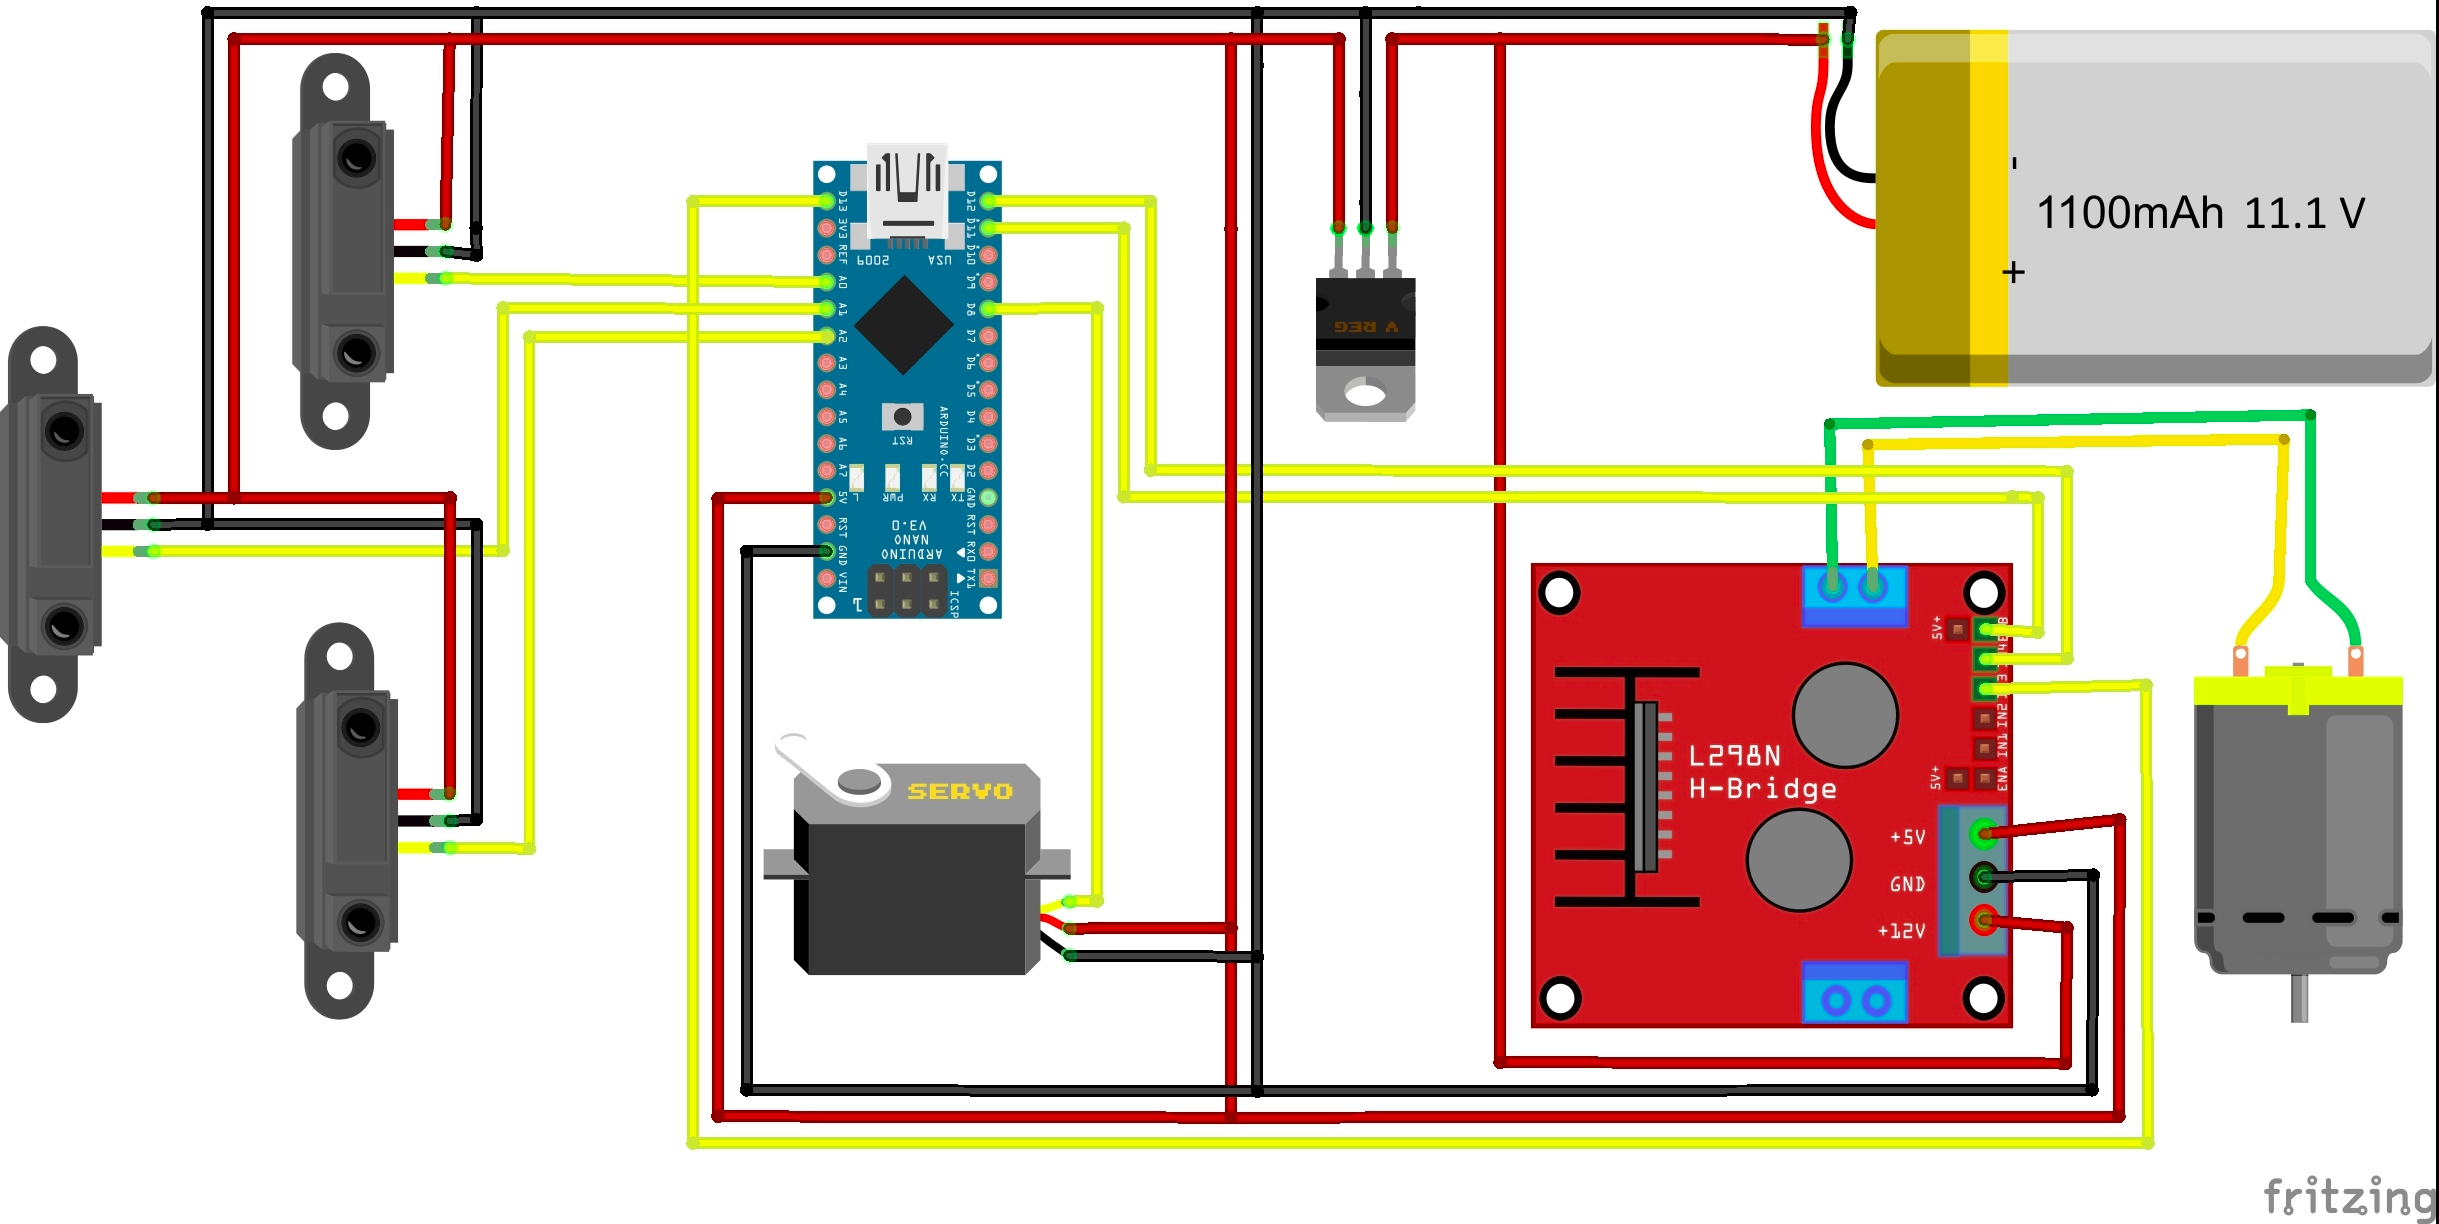
\includegraphics[width=10cm]{w_09_2016_Sklipus5.png}
  \caption {Общая схема робота}\label{Sklipus5}
\end{figure} 

\subsection*{Программирование робота}

Так как на роботе используется Arduino, то программирование выполняется с использованием Arduino IDE. Программа робота представляет собой замкнутый цикл, который состоит из следующих блоков:

\begin{enumerate}
  \item Фильтрация показаний датчиков;
  \item Вычисление угла и скорости движения робота;
  \item Передача управляющих сигналов на механизмы.
\end{enumerate}

В данной структуре отсутствует блок получения информации от датчиков. Так как датчики возвращают аналоговый сигнал, в Arduino IDE есть функция analogWrite(). Данная функция замечательно работает, если не важна скорость измерения. Но так как робот разрабатывался для соревнований, было принято решение вынести обработку датчиков в прерывание.

Все  платы Arduino, построенные на микроконтроллере ATmega, имеют возможность проводить измерения АЦП в автоматическом режиме. Нужно один раз настроить этот режим, а потом пользоваться полученными значениями. В результате контроллер постоянно проверяет датчики, не тратя на это процессорное время. Фильтрация показаний датчиков осуществляется медианным фильтром с окном в три элемента.

Для движения по трассе был выработан следующий алгоритм. Робот сравнивает расстояния до правой и левой стенки, и в соответствии с этим поворачивает колеса в нужное направление. Если впереди робота нет препятствий, скорость  увеличивается, но также уменьшается максимально возможный угол поворота колес. Это нужно для того, чтобы на прямых участках робот ехал более прямо. При обнаружении препятствия угол поворота колес увеличивается, и робот притормаживает.

Есть конечно и нерешенные проблемы. Например, робот не знает кривизну поворота, поэтому тормозит перед каждым поворотом.

Посмотреть код проекта можно на GitHub~\cite{Sklipus3}.

\begin{thebibliography}{99}

\bibitem{Sklipus1} \url{https://en.wikipedia.org/wiki/Servo\_\%28radio\_control\%29}
\bibitem{Sklipus2} \url{https://www.google.com/url?q=https\%3A\%2F\%2Fsites.google.com\%2Fsite\%2Fsklipusrobotsystems\%2Fhardware\%2Fpower-of-robot\&sa=D\&sntz=1\&usg=AFQjCNHdVp\_jzQoLmZ8pIL3PrrfXRarkuA}
\bibitem{Sklipus3} \url{https://github.com/sklipus/roborace/tree/master/robots/FreshSRDEDITION}
\end{thebibliography}

\end{document}
